\documentclass[a4paper,12pt]{article}

% Include support for english hyphenation (if installed on your sistem)
\usepackage[english]{babel}

% Include support for correct printing of romanian characters
\usepackage[T1]{fontenc}
\usepackage{ucs}
\usepackage[utf8x]{inputenc}

\hyphenpenalty 10000
\exhyphenpenalty 10000

% Include support for graphics
\usepackage{graphicx}

% Include support for figures
\usepackage{subfig}
\DeclareGraphicsExtensions{.pdf,.png,.jpg}

% Include support for color
\usepackage{color}

% Include support for code listing
\usepackage{listings}

% Include support for links
\usepackage{hyperref}
\hypersetup{
    colorlinks=false,
    pdfborder={0 0 0},
}

% Include support for inline figures
\usepackage{wrapfig}

% Make margins shorter 
%\usepackage{fullpage}
\usepackage[top=2.54cm,bottom=2.54cm,left=2.54cm,right=2.54cm]{geometry}
%\usepackage[top=3.81cm,bottom=3cm,inner=3.5cm,outer=2.54cm]{geometry}

% Indent paragraphs
%\setlength{\parindent}{8pt} 
%\parindent 8pt

% Indent firs paragraph in a section
\usepackage{indentfirst}

\usepackage{setspace}
\onehalfspacing
\begin{document}

 % the title pages
\begin{titlepage}
\title{Research on Arch Framework \\ How to Improve the Execution-Time \\ -PDCS Programming Project-  \\ -report-}
\author{Cristian Mihai Barca - cba390, 2514228 \\ Advisers: Jacopo Urbani, Ceriel Jacobs}
\date{20/01/2013}
\maketitle
\end{titlepage}


 %the short description of the thesis
 %\include{chapter0/abstract}
 
 \tableofcontents 
 %\listoffigures

\lstset{numbers=left, stepnumber=1, language=Java, tabsize=2} 

 %the first chapter
 % CHAPTER_BEGIN
\section{Ajira Framework: Research Report}

\subsection{Introduction}

The \textit{ajira} project is a custom made framework for writing mainly HPC data applications. It is built on top of IPL (Ibis Portability Layer - the communication layer) and embraces a master-slave architecture. The master is basically another worker that has the extra task to setup the communication and start splitting the work between all the nodes (the workers). Thus, we do not have to install and configure anything as a separate platform and then use a special API to run jobs/tasks on top of that platform (i.e such as using Hadoop). Instead, what we need to run such an application is the \textit{ibis-server} (embedded inside the \textit{ajira} framework so we can run it from there and have our communication layer up) and, of course, a program that uses \textit{ajira} for data computations. Usually, the program does not have to be divided into a master and slave architecture. We can only use \textit{ajira} framework to write the master section. The workers' behavior is automatically dictated by the list of actions we write in the code, inside the job's description. For testing my experimental changes on the project, I have used an Ajira application that sorts large data-sets of RDF triples. To run this entire setup (\textit{ajira} + \textit{sorting application}) I have used the git repository for code deployment on DAS4 and a self written \textit{ant} file \cite{build_file} to build the application into a .jar bundle package (a package that embeds all the necessary dependencies, including the \textit{ajira.jar} package built with the default provided ant file). Next, to run the \textit{sorting application} on DAS4 a simple \textit{prun} command execution (see next section) was used.

% 
\subsection{Deployment \& execution on DAS4}

For \textit{ajira's} and \textit{sorting application's} main-code deployment on DAS4 access to git repositories \cite{arch_repo}, \cite{qpie_repo} is required. Clone the repositories in your DAS4 home directory and be sure that you are located in the benchm\_master branch. For the entire list of steps that you have to follow in order to run/execute this setup on multiple nodes, see below.
\newline
\newline
\textbf{Steps for running the \textit{sorting application} on multiple DAS4 cluster nodes:}
\begin{enumerate}
	\item Deploy \textit{ajira} and the \textit{demo sorting application} projects in your DAS4 home directory. Each project already has all the dependencies and ant files needed to built it, 
	\item Build \textit{ajira} using its ant build file: 'ant build-jar',
	\item Copy the \textit{ajira.jar} file to the \textit{lib} directory of the \textit{sorting app},
	\item Build \textit{sorting app} project using its ant build file \cite{build_file}: 'ant build-jar' (this will create a .jar file that we use to execute its main class - BenchmarkSorting - on DAS4; the .jar is placed by default in the \textit{jar} directory -- for any changes look at the parameters inside the ant file)
	\item Configure \textit{ibis-server} parameters (port, enable events, etc) from inside \textit{ajira's} ant build file,
	\item Start \textit{ibis-server} on the DAS4 head-node from the \textit{ajira} project directory: 'ant ibis-server' (note the address and port that is using),
	\item Run/execute the bundle package on DAS4 using the script example \cite{run_on_das4} -- change the parameters for your own needs.
\end{enumerate}

% 
\subsection{Workflow example: how \textit{ajira} can be used to sort RDF triples}

In this section I will explain how \textit{ajira} works on 'crunching' data, using as an example the RDF triples' \textit{distributed sorting} implemented inside the \textit{sorting example application}. To begin with, the sorting process can be split in 3 steps: (1) read and sort RDF triples; (2) send-receive communication; (3) merge and write RDF triples in files;

The main data structure used for all of the steps is the \textit{'Bucket'} -- an in-memory buffer that is filled up with triples of which hash keys are equal to the bucket's identifier. When the buffer limit size is exceeded, all of its content gets sorted and cached on the hard-disk (in temporary files). Thus, when we refer to the 'Bucket' we usually mean both the in-memory buffer and the temporary files. Each time the files' number increases above a fixed limit, a thread starts and merges them 2-by-2 up until their number gets below this limit. All the information about the files (metadata such as names, first elements, size, etc) is kept inside the Bucket -- we need those when we transfer the triples or write the results. By default, each node keeps 1 bucket in memory for every other node (remote-buckets), including itself (local-bucket). So, there are by default N buckets on each node, where N = number of nodes; a new feature allows you to use more than 1 bucket per node (NPARTITIONS\_PER\_NODE parameter, which by default is 1). The creation and initialization of a bucket (create, get, release, etc) is controlled by the 'Buckets' wrapper class.

% 
\subsubsection*{(1) Read and sort the RDF triples}

First, the data set (compressed or not) gets split into file partitions of almost the same size and each partitions is assigned to a single node for reading. The data set split is done by the ReadFromFiles action, which creates FileCollections of a minimumFileSplitSize. Next, the FileLayer of each node reads the triples from its assigned partitions -- the FileCollections, a set of path names representing the location of the files that were partitioned -- and inserts them into the corresponding local/remote bucket (where the triple's hash key equals to the node's bucket id). When a bucket gets full with triples its content is sorted using the java's default MergeSort algorithm and then cached on the disk. All of the information/metadata about the disk caching is stored inside the Bucket object for further use. If there is no more data left to read from a partition the node broadcasts a signal, alerting that the remote-buckets are ready to be transferred (this means that the send-receive start point is dependent on the size of the file partition). See Figure~\ref{fig:diag1} for a better understanding. So, at this point, the send-receive step begins -- triples are transferred from the remote-buckets to their assigned nodes (i.e. on node Y, we have a remote-bucket for node X that has triples assigned to X; these triples will be transferred to X's local-bucket).

\begin{figure}
\centering
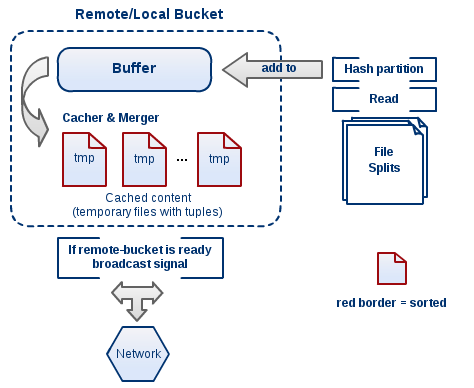
\includegraphics[scale=0.6]{diag1}
\caption{Read and sort - remote \& local buckets structure}
\label{fig:diag1}
\end{figure}

% 
\subsubsection*{(2) Send-receive communication}

When a signal alert for a bucket ready for transfer is received by a node (\textit{receiver}), a corresponding request for fetching the triples is sent back to the \textit{sender}. Then, the \textit{sender} registers that request and, whenever the remote-bucket has available data for transfer, removes a chunk and sends it to the \textit{requester}. Next, the \textit{recipient} adds that chunk into its local-bucket and \textit{sends} a request for another fetch. As long as on the \textit{sender} side the remote-bucket still contains triples, the \textit{receiver} will get chunks transferred to its local-bucket. If the remote-bucket is empty it is released and the transfer's metatada are cleaned/removed. Nevertheless, a last signal that marks the end of the transfer is sent to the \textit{recipient}, which flags its local-bucket with \textit{finished} -- meaning that is ready for merge \& write. In Figure~\ref{fig:diag2} we show very briefly the workflow of the send-receive communication. The chunk removal, in the worst case of triples getting cached on the disk, has to extract all the minimum triples from the in-memory buffer and cached files (in sorted order) up until it fills the chunk. Is it necessary to do that because we expect to receive sorted data on the \textit{recipient} side. Otherwise,  we send a chunk directly from the in-memory buffer, after we have sorted it.

\begin{figure}
\centering
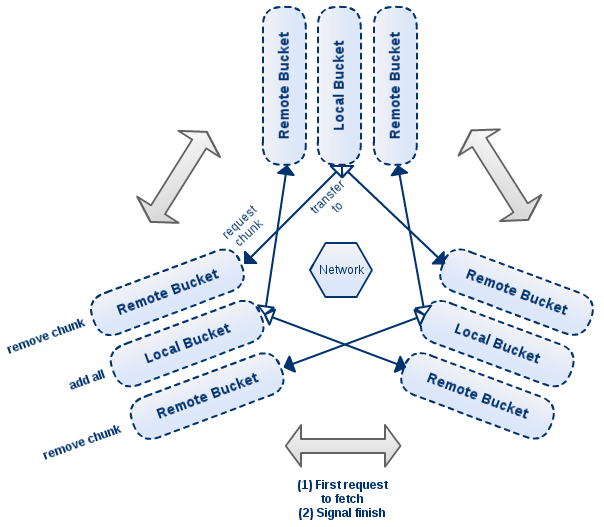
\includegraphics[scale=0.6]{diag2}
\caption{Transfer to correspondent nodes - send-receive communication}
\label{fig:diag2}
\end{figure}

% 
\subsubsection*{(3) Merge and write the RDF triples in files - results output}

When all the triples from the remote-buckets are sent (the previous step is finished), the final step merges the local-bucket's in-memory buffer with its cached content (the temporary files from the hard disk). This task is done by the same method (\textit{removeChunk()}) that removes chunks from a bucket. Now it fetches data from the local-bucket whenever the bucket-iterator is called to write data. In the end, the result of each node is represented by a single sorted RDF triples file per partition. This step is illustrated in Figure~\ref{fig:diag3}.

\begin{figure}
\centering
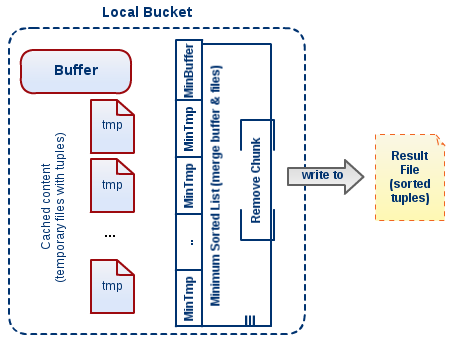
\includegraphics[scale=0.5]{diag3}
\caption{Merge and write}
\label{fig:diag3}
\end{figure}

\pagebreak

% 
\subsection{Execution-time}

Testing configuration: 
\begin{itemize}
	\item \textbf{Cluster-Node}: 1 Node @ DAS4, 16 x QuadCore Intel Xeon CPU E5620 @ 2.4GHz 
	\item \textbf{Number of Nodes}: 8, 12, 16
	\item \textbf{Dataset sizes}: 21, 38, 62, 149 GB
	\item \textbf{Split sizes}: 256MB, 1GB, 2GB, 4GB (0.5, 2, 4, 8 times the size of the memory buffer)
	\item \textbf{Common setups}: 512MB buffer size, available to transmit on 128MB (0.25 x buffer size), 8 concurrent tuple senders
\end{itemize}

Test - 8 nodes
\newline \newline
\renewcommand{\arraystretch}{1.2}
{\footnotesize\tt
\begin{tabularx}{\linewidth}{c|c|c|c|c|c|c|c|c|c|l}
\cline{2-10}
& SplitSz 
& \multicolumn{3}{c|}{256MB} & \multicolumn{3}{c|}{1GB}  & \multicolumn{1}{c|}{2GB} & \multicolumn{1}{c|}{4GB} \\
\cline{2-10}
& DataSz 
& 21 & 38 & 62 & 21 & 38 & 62 & 62 & 149 \\
\cline{2-10}
& 1
& 2m55.610s & 9m7.906s & 17m42.352s & 4m11.063s & 9m34.963s & 18m7.227s & 17m49.267s & 48m1.221s \\
\cline{2-10}
& 2
& 2m33.504s & 6m1.188s & 15m51.920s & 3m18.747s & 7m44.045s & 18m12.263s & 18m1.078s & 44m27.157s \\
\cline{2-10}
& 3
& 3m6.434s & 6m38.414s & 15m23.895s & 3m28.962s & 7m45.673s & 17m17.323s & 17m52.446s & 43m28.572s \\
\cline{2-10}
& 4
& 3m5.056s & 6m3.399s & 18m4.935s & 2m55.823s & 6m58.610s & 18m27.074s & 17m22.566s & 43m40.874s \\
\cline{2-10}
& 5
& 2m43.189s & 9m20.022s & 17m27.871s & 2m39.512s & 6m8.775s & 18m7.482s & 18m18.761s & 43m12.089s \\
\cline{2-10}
& 6
& 2m57.097s & 7m12.720s & 15m36.118s & 2m52.811s & 7m22.610s & 17m24.032s & 17m12.491s & 43m35.471s \\
\cline{2-10}
& 7
& 3m12.328s & 9m10.939s & 14m45.655s & 3m24.775s & 9m30.433s & 17m52.905s & 18m15.298s & 43m24.891s \\
\cline{2-10}
& 8
& 2m38.030s & 9m8.566s & 14m9.058s & 2m31.495s & 8m33.343s & 17m47.242s & 17m17.465s & 44m31.543s \\
\cline{2-10}
& 9
& 3m4.586s & 6m59.591s & 14m18.144s & 2m33.705s	& 9m15.151s & 17m31.529s & 16m49.083s & 46m54.699s \\
\cline{2-10}
& 10
& 3m1.391s & 6m42.639s & 15m24.180s & 2m38.665s & 8m12.664s & 18m16.361s & 18m8.805s & 46m22.130s \\
\cline{2-10}
& Avg (mm.ss)
& 2.92 & 7.63 & 15.86 & 3.04 & 8.1 & 17.9 & 17.7 & 44.75 \\
\cline{2-10}
\end{tabularx}

}

Test - 12 nodes
\newline \newline
\renewcommand{\arraystretch}{1.2}
{\footnotesize\tt
\begin{tabularx}{\linewidth}{c|c|c|c|c|c|c|c|c|c|l|}
\cline{2-10}
& SplitSz 
& \multicolumn{3}{c|}{256MB} & \multicolumn{3}{c|}{1GB}  & \multicolumn{1}{c|}{2GB} & \multicolumn{1}{c|}{4GB} \\
\cline{2-10}
& DataSz 
& 21 & 38 & 62 & 21 & 38 & 62 & 62 & 149 \\
\cline{2-10}
& 1
& 2m35.216s & 5m4.264s & 14m2.409s & 3m41.290s & 6m42.495s & 16m24.717s & 13m51.683s & 41m46.524s \\
\cline{2-10}
& 2
& 2m52.109s & 6m40.810s & 14m4.873s & 2m59.920s & 5m29.004s & 15m40.392s & 12m49.757s & 42m0.930s \\
\cline{2-10}
& 3
& 3m44.911s & 6m44.269s & 13m0.643s & 3m51.956s & 5m40.359s & 15m44.106s & 9m24.816s & 42m35.532s \\
\cline{2-10}
& 4
& 1m58.169s & 5m36.799s & 9m35.272s & 3m7.715s & 8m9.754s & 15m49.092s & 12m42.457s & 43m46.320s \\
\cline{2-10}
& 5
& 1m38.631s & 7m24.799s & 8m46.866s & 2m31.827s & 7m38.270s & 14m42.470s & 11m17.998s & 46m27.337s \\
\cline{2-10}
& 6
& 1m41.508s & 6m34.411s & 13m58.452s & 2m33.315s & 6m34.952s & 9m53.012s & 9m58.102s & 41m44.219s \\
\cline{2-10}
& 7
& 1m53.415s & 6m55.137s & 13m43.853s & 2m46.535s & 6m12.351s & 13m35.557s & 9m57.823s & 42m9.389s \\
\cline{2-10}
& 8
& 2m3.655s & 6m51.497s & 11m30.319s & 3m43.495s & 7m51.646s & 14m55.679s & 12m28.488s & 41m45.919s \\
\cline{2-10}
& 9
& 2m5.139s & 4m15.320s & 12m49.001s & 2m33.786s & 6m18.697s & 12m44.145s & 13m37.874s & 46m52.269s \\
\cline{2-10}
& 10
& 1m51.517s & 6m13.355s & 14m34.265s & 2m46.681s & 5m49.602s & 15m8.543s & 13m32.580s & 43m16.961s \\
\cline{2-10}
& Avg (mm.ss)
& 2.23 & 6.22 & 12.6 & 3.05 & 6.63 & 14.45 & 11.95 & 43.23 \\
\cline{2-10}
\end{tabularx}

}

Test - 16 nodes
\newline \newline
\renewcommand{\arraystretch}{1.2}
{\footnotesize\tt
\begin{tabularx}{\linewidth}{*{10}{c|}}
\cline{2-10}
& SplitSz 
& \multicolumn{3}{c|}{256MB} & \multicolumn{3}{c|}{1GB}  & \multicolumn{1}{c|}{2GB} & \multicolumn{1}{c|}{4GB} \\
\cline{2-10}
& DataSz 
& 21 & 38 & 62 & 21 & 38 & 62 & 62 & 149 \\
\cline{2-10}
& 1
& 1m49.319s & 3m33.105s & 11m50.674s & 2m23.195s & 6m48.559s & 17m20.231s & 9m36.172s & 42m41.332s \\
\cline{2-10}
& 2
& 1m42.915s & 3m10.699s & 9m12.623s & 2m37.009s & 6m2.826s & 16m33.021s & 8m21.347s & 39m33.850s \\
\cline{2-10}
& 3
& 1m40.766s & 5m25.910s & 13m20.892s & 2m1.783s & 5m53.417s & 16m8.924s & 10m1.235s & 38m41.223s \\
\cline{2-10}
& 4
& 1m32.892s & 3m5.498s & 9m55.324s & 2m14.099s & 5m6.707s & 13m5.015s & 10m45.445s & 38m5.924s \\
\cline{2-10}
& 5
& 1m32.807s & 4m2.091s & 9m13.591s & 2m16.201s & 5m8.894s & 13m39.965s & 11m21.077s & 40m15.218s \\
\cline{2-10}
& 6
& 1m42.776s & 3m23.211s & 10m16.718s & 1m44.661s & 4m24.347s & 12m23.631s & 11m25.137s & 38m28.968s \\
\cline{2-10}
& 7
& 1m32.122s & 5m22.415s & 7m52.420s & 2m21.044s & 5m19.627s & 14m27.422s & 11m23.863s & 37m55.466s \\
\cline{2-10}
& 8
& 1m52.346s & 2m48.023s & 7m59.697s & 1m44.995s & 4m13.464s & 13m49.629s & 6m30.170s & 38m2.429s \\
\cline{2-10}
& 9
& 1m41.379s & 5m8.554s & 10m22.603s & 1m47.492s & 4m28.210s & 12m54.858s & 8m7.309s & 37m10.927s \\
\cline{2-10}
& 10
& 1m49.002s & 5m16.802s & 12m47.414s & 2m34.393s & 4m4.019s & 10m56.675s & 9m29.239s & 37m52.524s \\
\cline{2-10}
& Avg (mm.ss)
& 1.68 & 4.12 & 10.27 & 2.16 & 5.14 & 14.12 & 9.69 & 38.87 \\
\cline{2-10}
\end{tabularx}

}

% 
\subsection{Proposals \& implementations: how to improve \textit{ajira's} \\ execution-time}

In general, a distributed large scale data application is considered optimal if each data-item (in our case \textit{1 single RDF triple}) is processed using less than (inclusive) 2 writes on disk \cite{tritonsort}. In the worst case, when dealing with a big amount of data (a file partition split size bigger than the size of our available memory), the total number of disk writes goes up to 3 (1 write for reading/sorting/caching data on the disk, 1 on the recipient side for gathering data in the local-bucket and  1 for writing the final results). Given the previous research I did on Hadoop's Map-Reduce \cite{hadoop}, a platform for processing data which has a layer for data partitioning \cite{shuffling} to the reducers, I came up with the following ideas: 
\begin{itemize}
\item to \textit{disable the local sorting of remote-buckets},
\item to \textit{start as soon as possible the triples' transfer/send-receive} (we do not need to keep data more than is necessary) and
\item to \textit{use an in-background double buffering mechanism to provide final merged chunks for the bucket-iterator}. 
\end{itemize}

These proposals aim to increase the chances of using less then 3 writes on disk (unless the network is a bottleneck) and to improve the execution time of the \textit{ajira} framework. From a distributed-sorting application point of view, this approach of moving the sort phase to the recipient side with the consequence of having less writes to disks may improve the total time of the execution. In the following paragraphs I will discuss each proposal and also provide some implementation aspects.

% 
\subsubsection*{(1) Disabling sort property for remote-buckets}

Because we start the up-call (data-transfer) at the moment we begin the read phase, we do not need to sort before-hand the remote-buckets. Instead, we apply the sorting on the recipient side (local-bucket), under the same assumptions -- when the buffer fills up, we sort and cache its content on the disk. To disable sorting on the remote-buckets, we have to construct/initialize them without the sorting function and sorting parameters.

% 
\subsubsection*{(2) Interleave the transfer with the local reading}

Due to the early start of the transfer, it is obvious that now the send-receive overlaps with the files-partition read phase. So, during the startTransfer() call we also have to broadcast signal alerts to the other nodes to have them send back requests for fetching data (the alertTransfer() method). To enable that we have to accomplish the followings:

\textbf{(a) Allow receiving of unsorted data}
Previously, when a chunk was transferred (\textit{sendTuples() method}) we specified the sorting function and its parameters in the message. Because we do not want to sort the remote-buckets anymore, we set a null sorting function and parameters. Thus, on the recipient side we have to allow the append of unsorted data into the local-bucket. The original version of \textit{addAll()} method, which adds chunks into the local-bucket, expected sorted data -- it compares the size of the chunk with the size of the buffer and depending on which one is bigger that one is cached on the disk (\textit{cacheBuffer() method}). If the chunk is bigger we cache directly without sorting (we already have done that on the sender side), otherwise we sort the buffer and spill it on the disk. This logic is now changed a bit -- we first try to add the chunk into the buffer, or the other way around if the buffer has fewer elements, instead of writing directly to the disk. Only if that fails, we sort and cache in a temporary file the bigger one. 

\textbf{(b) Split the main buffer into two buffers}

Furthermore, we can improve the previous idea by splitting the main buffer into two separate buffers in such way that one should be use for reading (\textit{inBuffer}) and one for receiving chunks (\textit{exBuffer}). With this approach, we can operate independently on each buffer. One disadvantage is that we require extra memory for the second buffer. At the end of the transfer -- when the bucket is flagged with finished -- we merge one buffer into the other (\textit{combineInExBuffers()} method) in order to have a single buffer combined with both information. If both are big, one of them (the smaller one) is cached on the disk.

\textbf{(c) Loosen-up the synchronization between bucket's methods}

Moreover, in addition to splitting the main buffer into two independent buffers, we can loosen-up the synchronization primitives between the read and transfer (\textit{add() and addAll() methods}), the only coarse synchronization point being the moment that both methods call \textit{cacheBuffer()} (both buffers might get full at the same time).

Steps 1 and 2 are described in Figure~\ref{fig:diag4}.

\pagebreak

\begin{figure}
\centering
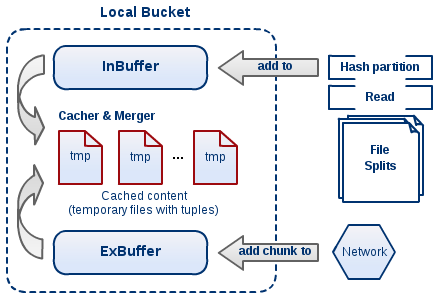
\includegraphics[scale=0.5]{diag4a}
\linebreak
\linebreak
\centering
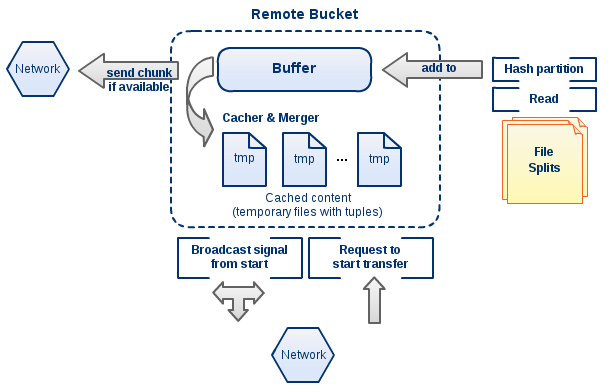
\includegraphics[scale=0.5]{diag4b}
\caption{New local/remote buckets}
\label{fig:diag4}
\end{figure}

% 
\subsubsection*{(3) Double-buffering for writing the results in files}

The last proposal concerns the writing of the sorted local-bucket (all the triples) into the final result file. This phase uses a \textit{bucketIterator} to iterate over the results. As in turn the iterator uses multiple \textit{removeChunk()} method calls to fetch chunks from the local-bucket when there are no more triples to iterate/write down. An idea would be to "hide" the time that the iterator has to wait for merging-up triples from the main memory (buffer) with the ones stored on the disk. Instead we can try to remove/get a chunk that has been already processed and stored in a set of auxiliary buffers in memory (triples ready to 'serve' the iterator). To implement this, we start a separate thread when we set the bucket's flag on finished, to fill up auxiliary buffers with chunks from the main buffer. When a write is performed the iterator is called and the chunk is taken directly from the auxiliary buffers instead of waiting for the whole merging phase. Moreover, when a buffer from the set empties the thread will go on and try to refill it, if there are triples available -- this mechanism of storing buffers that were pre-processed is called 'Double-Buffering'. Figure~\ref{fig:diag5} refers to \textit{removeChunk()} call mechanism explained in this paragraph. 

\begin{figure}
\centering
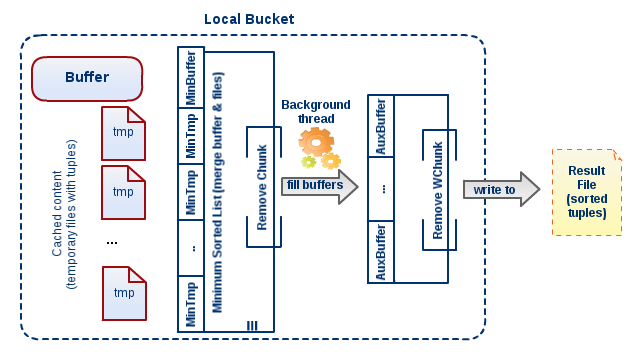
\includegraphics[scale=0.6]{diag5}
\caption{In-background merge-up}
\label{fig:diag5}
\end{figure}

% 
\subsubsection{Results: execution-time}

Test - 8 nodes
\newline \newline
\renewcommand{\arraystretch}{1.2}
{\footnotesize\tt
\begin{tabularx}{\linewidth}{*{10}{c|}}
\cline{2-10}
& SplitSz 
& \multicolumn{3}{c|}{256MB} & \multicolumn{3}{c|}{1GB}  & \multicolumn{1}{c|}{2GB} & \multicolumn{1}{c|}{4GB} \\
\cline{2-10}
& DataSz 
& 21 & 38 & 62 & 21 & 38 & 62 & 62 & 149 \\
\cline{2-10}
& 1
& 2m40.815s & 7m57.255s & 15m41.617s & 3m2.585s & 7m26.847s & 15m52.020s & 16m58.103s & 47m33.350s \\
\cline{2-10}
& 2
& 2m34.868s & 6m15.128s & 15m32.877s & 2m39.325s & 8m52.215s & 15m37.135s & 15m16.995s & 47m29.418s \\
\cline{2-10}
& 3
& 2m30.706s & 6m5.774s & 14m47.793s & 2m43.720s & 5m58.528s & 17m16.021s & 16m24.077s & 47m23.859s \\
\cline{2-10}
& 4
& 2m30.446s & 6m53.190s & 14m49.342s & 2m44.330s & 6m58.543s & 15m51.803s & 15m56.746s & 47m21.741s \\
\cline{2-10}
& 5
& 3m4.606s & 6m43.932s & 15m25.822s & 2m40.153s & 5m13.739s & 17m2.552s & 16m12.159s & 47m26.099s \\
\cline{2-10}
& 6
& 3m9.408s & 6m28.413s & 16m11.942s & 2m40.224s & 5m25.047s & 15m24.170s & 16m31.383s & 47m21.517s \\
\cline{2-10}
& 7
& 2m48.874s & 4m46.725s & 16m25.753s & 2m32.941s & 6m19.333s & 14m18.357s & 16m52.848s & 43m6.666s \\
\cline{2-10}
& 8
& 2m40.238s & 7m25.513s & 15m45.134s & 2m28.537s & 9m11.525s & 15m9.601s & 16m18.642s & 43m55.177s \\
\cline{2-10}
& 9
& 2m30.935s & 6m55.467s & 15m41.847s & 2m33.696s & 7m53.475s & 16m0.388s & 16m25.423s & 46m44.169s \\
\cline{2-10}
& 10
& 2m37.317s & 6m54.436s & 15m38.446s & 2m53.944s & 7m19.787s & 17m15.853s & 16m26.889s & 47m10.179s \\
\cline{2-10}
& Avg (mm.ss)
& 2.7 & 6.63 & 15.59 & 2.69 & 7.05 & 15.97 & 16.3 & 46.54 \\
\cline{2-10}
& Improv. \%
& 7.53 & 13.11 & 1.70 & 11.51 & 12.96 & 10.78 & 7.91 & -NONE- \\
\cline{2-10}
\end{tabularx}

}

\newpage

Test - 12 nodes
\newline \newline
\renewcommand{\arraystretch}{1.2}
{\footnotesize\tt
\begin{tabularx}{\linewidth}{c|c|c|c|c|c|c|c|c|c|l|}
\cline{2-10}
& SplitSz 
& \multicolumn{3}{c|}{256MB} & \multicolumn{3}{c|}{1GB}  & \multicolumn{1}{c|}{2GB} & \multicolumn{1}{c|}{4GB} \\
\cline{2-10}
& DataSz 
& 21 & 38 & 62 & 21 & 38 & 62 & 62 & 149 \\
\cline{2-10}
& 1
& 1m50.679s & 5m31.063s & 13m10.769s & 3m6.879s & 6m13.877s & 14m5.243s & 12m51.575s & 45m31.696s \\
\cline{2-10}
& 2
& 1m52.036s & 4m59.978s & 9m8.194s & 2m58.449s & 5m26.362s & 14m2.959s & 12m43.355s & 42m31.401s \\
\cline{2-10}
& 3
& 2m2.744s & 3m51.152s & 13m4.056s & 2m6.365s & 6m8.137s & 14m6.316s & 12m36.971s & 45m2.317s \\
\cline{2-10}
& 4
& 2m9.747s & 6m20.750s & 12m10.497s & 2m59.096s & 5m30.037s & 12m1.829s & 11m4.499s & 43m29.198s \\
\cline{2-10}
& 5
& 2m5.854s & 3m14.792s & 9m13.899s & 2m0.390s & 6m11.867s & 11m55.725s & 9m10.917s & 42m58.603s \\
\cline{2-10}
& 6
& 2m24.353s & 2m51.950s & 12m23.965s & 2m2.408s & 4m28.531s & 13m57.812s & 11m45.212s & 43m7.404s \\
\cline{2-10}
& 7
& 1m46.429s & 3m38.576s & 12m18.557s & 2m24.491s & 5m40.746s & 14m15.596s & 11m45.168s & 43m53.767s \\
\cline{2-10}
& 8
& 1m43.859s & 5m3.728s & 10m57.489s & 2m12.176s & 4m19.665s & 14m13.373s & 10m49.813s & 42m42.329s \\
\cline{2-10}
& 9
& 2m1.370s & 5m43.489s & 12m3.150s & 2m8.212s & 3m48.096s & 12m38.087s & 11m22.283s & 43m25.376s \\
\cline{2-10}
& 10
& 2m2.946s & 4m35.691s & 12m38.006s & 2m5.706s & 5m45.697s & 13m15.133s & 12m35.941s & 44m49.665s \\
\cline{2-10}
& Avg (mm.ss)
& 2 & 4.57 & 11.7 & 2.4 & 5.34 & 13.44 & 11.66 & 43.74 \\
\cline{2-10}
& Improv. \%
& 10.31 & 26.53 & 7.14 & 21.31 & 19.46 & 6.99 & 2.43 & -NONE- \\
\cline{2-10}
\end{tabularx}

}

Test - 16 nodes
\newline \newline
\renewcommand{\arraystretch}{1.2}
{\footnotesize\tt
\begin{tabularx}{\linewidth}{*{10}{c|}}
\cline{2-10}
& SplitSz 
& \multicolumn{3}{c|}{256MB} & \multicolumn{3}{c|}{1GB}  & \multicolumn{1}{c|}{2GB} & \multicolumn{1}{c|}{4GB} \\
\cline{2-10}
& DataSz 
& 21 & 38 & 62 & 21 & 38 & 62 & 62 & 149 \\
\cline{2-10}
& 1
& 1m41.969s & 3m49.298s & 13m55.218s & 2m36.927s & 6m4.237s & 10m39.667s & 8m48.566s & 40m37.759s \\
\cline{2-10}
& 2
& 1m40.338s & 3m47.789s & 13m19.358s & 2m1.960s & 5m24.346s & 12m40.292s & 9m17.997s & 37m54.868s \\
\cline{2-10}
& 3
& 1m39.998s & 2m55.300s & 13m40.155s & 2m2.099s & 5m38.308s & 13m1.947s & 7m57.156s & 38m20.263s \\
\cline{2-10}
& 4
& 1m32.664s & 4m10.906s & 13m12.273s & 1m49.085s & 6m28.060s & 13m17.127s & 9m3.974s & 37m43.711s \\
\cline{2-10}
& 5
& 1m31.912s & 3m23.316s & 10m36.658s & 2m2.151s & 4m41.135s & 11m55.222s & 6m19.858s & 41m32.575s \\
\cline{2-10}
& 6
& 1m30.868s & 3m20.186s & 14m11.719s & 2m17.648s & 5m0.436s & 13m16.737s & 6m2.039s & 40m37.573s \\
\cline{2-10}
& 7
&  1m31.340s & 5m5.723s & 13m0.218s & 2m19.167s & 5m35.444s & 12m24.751s & 4m13.467s & 37m54.181s \\
\cline{2-10}
& 8
& 1m26.041s & 5m1.699s & 12m32.280s & 2m27.565s & 6m4.404s & 12m32.675s & 9m56.222s & 37m59.779s \\
\cline{2-10}
& 9
& 1m28.403s & 4m23.519s & 10m58.033s & 1m59.172s & 4m47.506s & 13m15.030s & 8m57.491s & 37m3.179s \\
\cline{2-10}
& 10
& 1m43.837s & 3m41.606s & 12m5.290s & 2m11.033s & 4m25.160s & 11m9.291s & 6m46.095s & 34m2.013s \\
\cline{2-10}
& Avg (mm.ss)
& 1.56 & 3.95 & 12.74 & 2.17 & 5.41 & 12.41 & 7.73 & 38.36 \\
\cline{2-10}
& Improv. \%
& 7.14 & 4.13 & -NONE- & -NONE- & -NONE- & 12.11 & 20.23 & 1.31 \\
\cline{2-10}
\end{tabularx}

}

\newpage

Speedup test: average on the best 10 execution-times (mm.ss), see Figure~\ref{fig:speedup}
\newline \newline
\renewcommand{\arraystretch}{1.2}
{\footnotesize\tt
\begin{tabularx}{\linewidth}{*{7}{c|}}
\cline{2-7}
& DataSz|SplitSz
& \multicolumn{5}{c|}{38GB|256MB} \\
\cline{2-7}
& NumNodes
& 1 & 2 & 4 & 8 & 16 \\
\cline{2-7}
& Ajira
& 41.33 & 27.03 & 14.24 & 8.27 & 5.24 \\
\cline{2-7}
& Ajira-Research
& 38.54s & 22.52 & 14.3 & 8.1 & 4.02 \\
\cline{2-7}
\end{tabularx}

}

\begin{figure}
\centering
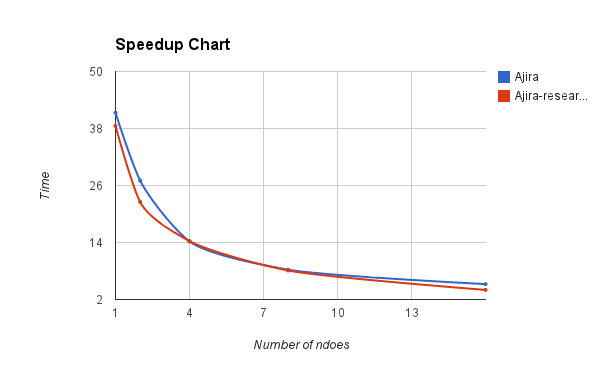
\includegraphics[scale=0.6]{speedup}
\caption{Speedup-chart for Ajira[blue] \& Ajira-Research[red]}
\label{fig:speedup}
\end{figure}

% 
\subsubsection*{Discussion}

What can we reason from the time results and improvement percentages is that there is an actually trade-of in performance between starting the transfer as soon as possible and starting after we read the first split of files (many small transfers, less to no W to disk VS. less bigger transfers, moderate to many W to disk). Notably, it depends a lot on the right parameter tuning over the cluster setup (network vs. storage, which one is faster?). Comparing the first two tables (8 and 12 nodes with 8 concurrent tuple senders) and also taking into account the speedup chart, we notice that our improvement increases for  tests with a 256MB and 1GB file split sizes and data set up to a 62GB size. Unfortunately, we cannot say the same about 62GB or a bigger data set and split size where we obtained a lower or even no improvements over the original version of Ajira. One possible cause would be that for 8 - 12 nodes a 4GB split size does not add an big overhead when we sort a data set of 149GB. We do have to wait for reading a 4GB file split (file partition) before starting the transfer, but for a 35x times bigger dataset and only for 8 - 12 nodes that is not overwhelming. In contrast, on the last table we achieved exactly the opposite. On the first 5 columns, 8 concurrent tuple senders for 16 nodes seems not to be enough to overcome the overhead caused by the file split. In this case the overhead is almost nonexistent because the tuples partitioning happens between more nodes than the previous tests. On the other hand, we see an increase of improvement over the last 3 columns, meaning that it makes sense not to wait for all 16 nodes to finish their 2GB - 4GB file partition read. 

\subsection{Future work}

For future work I propose the following developments:

\begin{itemize}
	\item \textit{Moving to processes.} One idea is to implement an option/feature that allows specifying how many 'instances' of PartitionToNodes to run locally and how many remotely on other nodes (following the Apache design model, i.e multiple mappers on same node). Example: if 1 node has 4 x QuadCore CPUs --- in total we can run 8 instances at least (maximum 16), 2 local instances on every node (given the fact that one instance makes highly use of multi-threading is fair enough to start only 2 processes per node).
	\item \textit{Thread synchronization.} In the Ajira framework we use threads for background processing and all the methods tend to be globally synchronized to avoid race conditions on the data structures. This adds a significant overhead to the application, because the access to the data structures becomes coarse grained. A solution for that is to use fine-grained/lock-free data structures or a mechanism such as double buffering. 
	\item \textit{Fine-grained file splitting.} In Ajira we coarsely split the data set between nodes. That means we consider an entire file when we decide where to send it (in what split collection), for further computations, instead of splitting the file in multiple pieces (i.e 64MB) and take their sizes into consideration. For small size files (with an order of maximum tens of MB) the coarse grained level works fine, but if the dataset has bigger files in small numbers we can get into an unbalanced situation.
	\item \textit{Data sampling.} Currently, the output of a distributed sorting application is not globally ordered. It means that we still have to merge each result file in order to get a full sorted data set from start to its end. Instead, a well known method to achieve global ordering and also fair data balancing is to perform a previous step called \textit{sampling}. A state-of-the-art idea is to rely on a Trie (a prefix tree) based algorithm with a depth level fixed in a way that will assure you enough granularity to equally balance the key partitions to all your nodes. When the tree is computed it can be used as a tuple partitioner instead of a hash algorithm in your normal data computation. An example of a Trie based sampling algorithm applied with Hadoop Map-Reduce is described in \cite{terasort}.
\end{itemize}

\subsection{Conclusions}

\begin{itemize}
	\item For batch processing of huge amount of data is still better to use the hard-disk to improve the execution time -- IO bound. So, what it matters now is how fast and when we should perform R/W operations comparing with other frameworks. On the other hand, for real-time processing the research approach is a better match -- network bound (not the case for distributed sorting which is an example of a batch processing).
	\item Probably an adaptive mechanism -- changing the file split size limit depending on the data set size automatically or exposing that to the user's decision -- would cover both explained scenarios
	\item Finally, both approaches got decent time executions and scaling-out performances for small, moderate and bigger data sets. Nevertheless, there is still space for further optimization. 
\end{itemize}

% CHAPTER_END
 \begin{thebibliography}{99}
	\bibitem{build_file}
		{\emph{Querypie} ant build file: \url{http://github.com/jrbn/querypie-storage/blob/safe_qpie/build.xml}}
	\bibitem{arch_repo}
		{\emph{Arch/Ajira} git repository: \url{https://github.com/jrbn/ajira} -- 'master' branch}
	\bibitem{qpie_repo}
		{\emph{Querypie} git repository: \url{https://github.com/jrbn/querypie-storage} -- 'master' branch}
	\bibitem{run_on_das4}
		{Example of bash script to run \emph{querypie} on DAS4: \url{http://gist.github.com/4585904}}
\end{thebibliography}

 
\end{document}